% --- COMMANDS ---
\makeatletter
\define@key{entry}{sound}[]{\def\entry@sound{#1}}
\define@key{entry}{pos}[]{\def\entry@pos{#1}}
\define@key{entry}{etym}[]{\def\entry@etym{#1}}
\define@key{entry}{note}[]{\def\entry@note{#1}}

\setkeys{entry}{sound,pos,etym,note}

% % digital-style definitions
% \newcommand{\entry}[3][]{%
% \begingroup%
% \setcounter{sense}{1}%
% \setkeys{entry}{#1}%
% \par \begin{minipage}{\columnwidth}%
% 	\textbf{\rzc #2}%
% 	\enskip {\footnotesize \ifdefempty{\entry@sound}{}{• \entry@sound{} nbm.} \ifdefempty{\entry@pos}{}{• \entry@pos}} \\%
% 	\ifdefempty{\entry@note}{}{\enskip {\footnotesize \textit{note:} \entry@note} \\}%
% 	\ifdefempty{\entry@etym}{}{\enskip {\footnotesize ← from \entry@etym} \\}%
% 	#3\vspace{12pt}%
% \end{minipage}%
% \endgroup%
% }

%\newcounter{sense}
%\NewDocumentCommand{\sense}{o}{%
%\ifnum\the\value{sense}>1\\\fi%
%	\textbf{\arabic{sense}:}\enskip%
%	\IfNoValueTF{#1}{}{\textit{#1}}%
%\stepcounter{sense}%
%}

% print-style definitions
% \newcommand{\entry}[3][]{%
% \begingroup%
% \setcounter{sense}{1}%
% \setkeys{entry}{#1}%
% \par \begin{minipage}{\columnwidth}%
% 	\textbf{\rzc #2}%
% 	\ifdefempty{\entry@pos}{}{\enskip•\enskip {\footnotesize\it\entry@pos}}%
% 	\ifdefempty{\entry@sound}{}{\enskip•\enskip {\footnotesize\entry@sound}}%
% 	\ifdefempty{\entry@etym}{}{\enskip←\enskip {\footnotesize\entry@etym}}%
% 	\ifdefempty{\entry@note}{}{\enskip•\enskip {\footnotesize\entry@note}}%
% 	\enskip•\enskip#3%
% \end{minipage}%
% \endgroup%
% }

% \newcounter{sense}
% \NewDocumentCommand{\sense}{o}{%
% \ifnum\the\value{sense}>1\enskip\fi%
% 	\textbf{\arabic{sense}}\enskip%
% 	\IfNoValueTF{#1}{}{\textit{#1}}%
% \stepcounter{sense}%
% }

\newcommand{\entry}[3][]{%
\begingroup%
\setcounter{sense}{1}%
\setkeys{entry}{#1}%
\par \begin{minipage}{\columnwidth}%
	\textbf{\rzc #2}%
	\ifdefempty{\entry@pos}{}{ • {\footnotesize\it\entry@pos}}%
	\ifdefempty{\entry@sound}{}{ • {\footnotesize\entry@sound}}%
	\ifdefempty{\entry@etym}{}{ ← {\footnotesize\entry@etym}}%
	\ifdefempty{\entry@note}{}{ • {\footnotesize\entry@note}}%
	\ • #3%
\end{minipage}%
\endgroup%
}

\newcounter{sense}
\NewDocumentCommand{\sense}{o}{%
\ifnum\the\value{sense}>1 \fi%
	\textbf{\arabic{sense}} %
	\IfNoValueTF{#1}{}{\ {#1}}%
\stepcounter{sense}%
}

\makeatother

\setchapterpreamble[u]{\margintoc}
\chapter{Lexicon}
A \langname{}-to-English dictionary is provided below.

\section*{How to use}
Entries for lexical items are listed by their spelling in generic form, ignoring morphophonological alterations. Derived words are listed as separate entries, but their source word is given. On the other hand, idiomatic or fixed expressions are given under the lexical item.

Each sense of a word has three basic parts: a quick, single-word translation for ease-of-use; a more detailed explanation of the concept; and an example sentence. The sentences are usually designed to help the reader figure the word's meaning out from context, particularly for \langname{} speakers and learners.

Pronunciations are given dictionary-style in a phonetic alphabet more intuitive to native \langname{} speakers.

\pagelayout{wide}
\setlength{\columnsep}{30pt}
\begin{multicols}{2}

% ===== A =====
\addsec{A}
\entry[pos=noun,sound=/ĕsyisŏíkli/]{asyisaikli}{\sense organization, association, official body}
\entry[pos=noun,sound=/avą́rĕ/,etym={OL₂ \pz{agą̆ré}, CC \fz{gamrī}},note=see \rz{secya}]{avąra}{\sense[ntr.] star or constellation used for navigation}
\entry[pos=noun,etym=Farlands \fz{rmḗdas}]{Arméds}{\sense[ntr.] the Gospels; a collection of poems sacred to the {\rzc Véajan} religion}

% ===== Ą =====
\addsec{Ą}
\entry[pos=noun,sound=/ǫ̆kássŏr/,etym=OL₂ \pz{ǫ̆kássŏr} “payment craft”]{ąkassar}{\sense[ntr.] mathematics}

% ===== C =====
\addsec{C}

% ===== E =====
\addsec{E}
\entry[pos=particle]{egi}{\sense just, only: \rz{egi matkó aczé sém lar tę-het} “she says there'll be just two baskets”}
\entry[pos=noun]{emas}{\sense[ntr.] plot of land}
\entry[pos=noun,etym=\rz{emas} + \rz{-soi}]{emassoi}{\sense boss; mid-level employee that oversees other employees \sense coach, manager, trainer; person with authority over a sports teams or its players  \sense[\bf\rzc emassoi kąstezi] coach; sports executive that makes substitutions and decides strategy \sense[\bf\rzc emassoi ǫkas] general manager; sports executive that signs and trades players \sense[archaic] feudal lord}
\entry[pos=adj.]{esyi}{\sense good \sense correct, appropriate}
% \entry[pos=noun,etym=\rz{esyi} + \rz{-soi}]{esyisoi}{}

% ===== Ę =====
\addsec{Ę}

% ===== F =====

% ===== H =====
\addsec{H}
\entry[pos=verb tr.,sound=/hŏssúsar/,etym={OL₂ \pz{hŏs-húsăr}, redup. of \pz{húsăr}}]{hassusar}{\sense exalt, praise (smn.)\sense[refl.] boast about \rz{tę} smth. \sense be a fan of, root for, cheer for (a team)}
\entry[pos=noun]{hakra}{\sense battle, skirmish \sense[pl.] military campaign \sense[pl.] semester}
\entry[pos=noun,etym=\rz{hakra} + \rz{-if}]{hakraif}{\sense field hockey; a ball game played on a pitch between two teams of seven, each attempting to win by scoring more points via goals than the opponent}
\entry[pos={verb tr.}]{husar}{\sense compliment \sense[archaic] shout at}

% ===== I =====
\addsec{I}
\entry[pos=noun,sound=/ístŏ/,etym={Farlands \fz{ī́sto}, \fz{hī́sto}}]{ista}{\sense[(\rz{Véajan}) ntr.] grace; a quite prayer ceremony for blessing food, travel, and other small events \sense[\rzc\bf tahąt osc-ista] give grace \sense[\rzc\bf fala ista] chamomile tea; a kind of soothing herbal drink imported from the Farlands} % \sense[{ntr. pl., poetic}] serenity, internal peace 

% ===== K =====
\addsec{K}
\entry[pos=noun,sound=/kĕ(n)gę́să/,etym={OL₂ \pz{kę̆kę́să}, redup. of \pz{kę̆să}}]{kagęsa}{\sense battalion, unit \sense army; a branch of the military comprising ground troops \sense[sports] team, club}
\entry[sound=/kę́stĕt/,pos=verb tr.]{kęstat}{\sense lead (smn.) towards \rz{tę} a goal \sense command: \rz{nassoin kęstací su kagęsa su kagę́staspa} “the king commands both army and navy.” \sense train (an apprentice) in \rz{tę} a skill: \rz{tę-coryam kęstatrí rat lala} “auntie's teaching me to sew.” \sense formally teach (a student) in \rz{ez} a discipline: \rz{rappahan picí kąstetnal ez-latya} “the minister was brought up in the faith.”}
\entry[pos=noun]{kęsa}{\sense soldier \sense[literary] protagonist, hero}

% ===== L =====
\addsec{L}

% ===== M =====
\addsec{M}
\entry[pos=noun]{mazzi}{\sense ballplayer}

% ===== N =====
\addsec{N}
\entry[pos=noun,sound=/náhhŏr/,etym=OL₂ \pz{náhhŏr} “gem craft”]{nahhar}{\sense[ntr.] ring, hoop \sense[ntr.] bracelet, bracer \sense[ntr. obs.] jewelry}
% \entry[pos=noun,sound=/nevĕ(n)díŏ/,etym=Farlands \fz{niēbendio}]{nevadia}{\sense[(\rz{Véajan}) ntr.] funeral; a prayer ceremony wishing a good afterlife, ending in a burial \sense[{\rzc\bf navediazi} derogatory] believer of {\rzc Véajan}}

% ===== O =====
\addsec{O}

% ===== Ǫ =====
\addsec{Ǫ}
\entry[pos=noun]{ǫkas}{\sense[ntr.] payment}

% ===== P =====
\addsec{P}
\entry[pos=noun,sound=/pălát(ă)s/]{palác}{\sense[ntr.] dinner}
\entry[pos=noun,etym=pormanteau of \rz{pakna u-palác},sound=/paknălát(ă)s/]{paknalác}{\sense inn, motel; short-term lodgings for a traveller between urban areas}

% ===== R =====
\addsec{R}

% ===== S =====
\addsec{S}
\entry[pos=noun,etym=compounding of \rz{sem véaja},note=always \sc prox]{Samvéajan}{\sense[ntr.] the Gospels; a collection of poems sacred to the {\rzc Véajan} religion}
\entry[pos=verb tr.]{sem}{\sense say to, talk to \sense[refl.] tell that \sense[refl.] say \sense[\rzc\bf sem ???] talk, speak \sense[coll., intr.] talk, speak \sense speak on, give an opinion on smth. concerning \rz{ez} \sense[\rzc\bf sem véaja] preach on \rz{ez} \sense[\rzc\bf sem ???] give a speech about \rz{ez} \sense[\rzc\bf sem ???] lecture on \rz{ez} \sense want smn. to \rz{im} do \sense[refl.] want to \rz{su} do \sense[\rzc\bf sem tę] would \sense[\rzc\bf sem tę] ought \sense[\rzc\bf sem tę] hopefully \sense[(of symbols, texts)] signify \sense[(of words, phrases)] mean, be defined as \sense[(of title, roles)] enable, allow to \sense[{\rzc\bf sagí tę} coll., refl.] let's go to \rz{tę}: \rz{sagí tę-tesan} “let's go to the beach” \sense[{\rzc\bf sagí tę} coll., refl.] let's \rz{tę} do: \rz{sagí tę-kęstat lala} “let's hire a nanny” \sense[coll.] looks like smn. \sense[{\rzc\bf samés} coll., intj.] looks like!}
% \entry[pos=verb tr.]{sem}{\sense say to, talk to \sense[(refl.)] tell that \sense[(refl.)] say \sense[\rzc\bf sem ???] talk, speak \sense[(coll., intr.)] talk, speak \sense speak on, give an opinion on \tsc{p} concerning \rz{ez} \sense[\rzc\bf sem véaja] preach on \rz{ez} \sense[\rzc\bf sem ???] give a speech about \rz{ez} \sense[\rzc\bf sem ???] lecture on \rz{ez} \sense want \tsc{p} to \rz{im} do \sense[(refl.)] want to \rz{su} do \sense[\rzc\bf sem tę] would \sense[\rzc\bf sem tę] ought \sense[\rzc\bf sem tę] hopefully \sense[(of symbols, texts)] signify \sense[(of words, phrases)] mean, be defined as \sense[(of title, roles)] enable, allow to \sense[{\rzc\bf sagí tę} (coll., refl.)] let's go to \rz{tę}: \rz{sagí tę-tesan} “let's go to the beach” \sense[{\rzc\bf sagí tę} coll., refl.] let's \rz{tę} do: \rz{sagí tę-kęstat lala} “let's hire a nanny” \sense[(coll.)] look like \tsc{p} \sense[{\rzc\bf samés} (coll., intj.)] looks like!}
\entry[pos=noun,etym={clipping of \rz{tahęnhar asyisaikli} “associated tag”}, note=see \rz{tahęnhar}]{sisik}{\sense[Inland] tag }

% ===== T =====
\addsec{T}
\entry[pos=verb in.,sound=/táhę̆t/]{tahąt}{\sense stretch (one's limbs) \sense reach for \rz{tę} something (to grab it) \sense aspire to \rz{tę} a difficult goal: \rz{tę-mazzi im-ot tahącí sec, manacan acoan raksí otnal kers} “he aspired to be a ballplayer, but he wasn't tall enough” \sense pray about \rz{osc} smth.}
\entry[pos=noun,sound=/tăhę́nhŏr/,etym=OL₂ \pz{tahę̆náhhŏr} “hoop reach”]{tahęnhar}{\sense[ntr.] tag; a parkour game played on an obstacle course between two teams over a number of rounds, each attempting to win by grabbing rings before being tagged 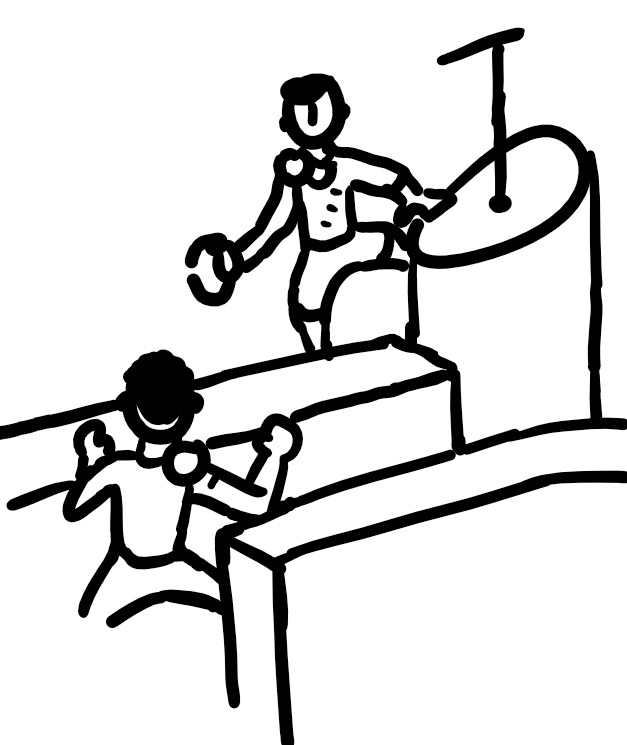
\includegraphics[width=\columnwidth]{sisik.png}}
\entry{taspa u-tesa}{\sense[idiom] kingdom}
\entry[pos=noun]{tesa}{\sense shoreline, bank; where a moving body of water meets the land \sense[of people] hair line}
\entry[pos=noun,sound=/teukkánŏs/,etym=Farlands \fz{tiēkᵛkános}]{teukkanas}{\sense[(\rz{Véajan}) ntr.] missionary, pastor; travelling evangelist who starts local chapters of faith centers \sense[humorous] tourist, vacationer}

% ===== U =====
\addsec{U}

% ===== V =====
\addsec{V}
\entry[pos=noun,sound=/véă(n)jŏ/,etym=Farlands \fz{vḗzșā}]{véaja}{\sense[ntr.] karma; recompense for virtuous behavior \sense[ntr. pl. prox.] a minority religion characterized by proselytization and belief in an afterlife \sense[\rzc\bf sesam véaja] preach, orate: \rz{rappahan sesamzí véaja ez-ǫkas esyi tę-laczin} “the minister preached of an eternal reward for the faithful”}

% ===== Y =====
\addsec{Y}
\entry[pos=noun,sound=/yerrŏ(n)gín/,etym={OL₂ \pz{yer-vŏngín}, Farlands \fz{iēlunzșín}}]{yerragín}{\sense[(\rz{Véajan}) ntr.] a prayer ceremony for greeting a visitor as a show of hospitality \sense[\rzc\bf tahąt osc-yerragín] lead the prayer ceremony \sense[idiom \rzc\bf yiat yerragín] show off, grandstand, put on airs: \rz{egi cuvarąn yiací yerragín tę-ahka im-nassoin} “the king knew the jester was only showing off”}

% ===== Z =====
\addsec{Z}

\end{multicols}